\section{随机试验}
\label{sec:cprob-experiments}

掷一枚骰子之前，我们不知道会出现几点，却清楚地知道只可能是$1,2,\ldots,6$中的一个。摸球、抽牌、抽检产品都有同样的结构：结果事先不确定，但全部可能结果事先可以列出。要谈“可能性有多大”，先要说清“什么的可能性”，也就是把可能结果和我们关心的问题写成数学对象。

\paragraph{样本空间与样本点}
在相同条件下可以重复进行、每次恰好产生一个结果、而全部可能结果事先已知的试验，称为\term{随机试验}（random experiment）。掷骰子、从盒中摸球、从一副牌中抽牌都是随机试验。一次试验究竟产生哪个结果事先不知道，概率要描述的正是这种不确定性。

\begin{definition}[样本空间与事件]
\label{def:cprob-sample-space}
随机试验全部可能结果组成的集合称为\term{样本空间}（sample space），记为$\Omega$，其元素$\omega$称为\term{样本点}（sample point）。样本空间的子集称为\term{事件}（event）。本章只讨论有限的样本空间，此时$\Omega$的每个子集都是事件。
\end{definition}

掷一枚骰子时，$\Omega=\{1,2,3,4,5,6\}$，“出现偶数点”是事件$\{2,4,6\}$，“点数大于$4$”是事件$\{5,6\}$。事件只是满足某个条件的那些结果放在一起，条件可以用文字说，也可以把元素列出来，两种写法指同一个集合。

整个样本空间$\Omega$也是事件，它包含全部结果，每次试验都发生，称为\term{必然事件}（certain event）。空集$\varnothing$不含任何结果，从不发生，称为\term{不可能事件}（impossible event）。只含一个样本点的事件$\{\omega\}$称为\term{基本事件}（elementary event）。

\paragraph{实际结果与事件}
试验做完以后，实际出现的是一个确定的样本点$\omega$。事件则是事先提出的问题，例如“会不会出现偶数点”。若实际结果$\omega\in A$，就说事件$A$在这次试验中\emph{发生}了，否则说它没有发生。

两者的区别在于数量。一次试验只产生一个结果，却可以同时让许多事件发生。设骰子掷出了$4$，那么$\{2,4,6\}$、$\{4,5,6\}$、$\{4\}$和$\Omega$都发生了，$\{1,3,5\}$和$\{5,6\}$没有发生。概率是对事件提出的，它在试验之前就有意义；试验之后，每个事件只剩下“发生”或“没发生”两种状态。

\paragraph{事件的运算}
事件既然是集合，集合运算就对应事件之间的逻辑组合，集合的记号可参考\BookChapterRef{chap:sets-relations-maps}{卷一第1章“集合、关系与映射”}。设$A,B$是事件：
\begin{itemize}
 \item 并$A\cup B$表示“$A$与$B$至少有一个发生”；
 \item 交$A\cap B$表示“$A$与$B$同时发生”；
 \item 补$A^{\mathrm{c}}=\Omega\setminus A$表示“$A$不发生”；
 \item 差$A\setminus B=A\cap B^{\mathrm{c}}$表示“$A$发生而$B$不发生”。
\end{itemize}

把$\Omega$画成矩形，把事件画成其中的区域，这些运算就是区域的合并、重叠和剩余，如图~\ref{fig:cprob-event-operations}所示。De Morgan律
\[
 (A\cup B)^{\mathrm{c}}=A^{\mathrm{c}}\cap B^{\mathrm{c}},\qquad
 (A\cap B)^{\mathrm{c}}=A^{\mathrm{c}}\cup B^{\mathrm{c}}
\]
读作：“至少一个发生”的反面是“两个都不发生”，“两个同时发生”的反面是“至少一个不发生”。后面计算“至少一个”时，常借这条规律转到它的反面。

\begin{BookInlineFigure}
  \centering
  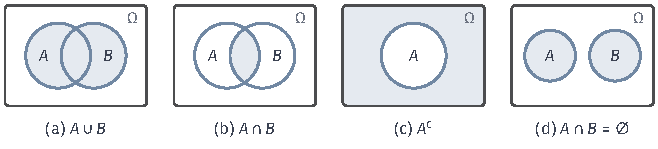
\includegraphics[width=112mm]{figures/07-probability/01-elementary-probability/tikz/cprob-event-operations/figure.pdf}
  \caption{事件的运算。矩形是样本空间$\Omega$，圆是事件，浅蓝区域是运算得到的事件。(a)并；(b)交；(c)补；(d)两个没有公共结果的事件。}
  \label{fig:cprob-event-operations}
\end{BookInlineFigure}

若$A\cap B=\varnothing$，即$A$与$B$没有公共的结果，就称它们\term{互斥}（mutually exclusive），如图~\ref{fig:cprob-event-operations}(d)。互斥的事件不能在同一次试验中同时发生。掷骰时“出现偶数点”与“出现$1$点”互斥；“出现偶数点”与“点数大于$4$”不互斥，结果$6$同时属于二者。

\paragraph{记录方式决定样本空间}
同一个物理过程可以用不同的方式记录，记录方式不同，样本空间就不同。下面用一个摸球问题说明这一点，本章后面会反复回到它：盒中有$5$个球，编号$1,2,3$的是黑球，编号$4,5$的是白球，搅匀后不放回地依次摸出两个。

第一种记录是按先后写下两个球的编号，结果是有序对$(a,b)$，$a\neq b$。第一个球有$5$种可能，第二个球有$4$种，样本空间有$5\times4=20$个点。第二种记录只写下摸到了哪两个球，不管先后，结果是二元子集$\{a,b\}$，共$\binom52=10$个。第三种只记颜色，结果是“黑黑”“黑白”“白黑”“白白”四种。

图~\ref{fig:cprob-urn-records}把三种样本空间并排画出。事件“两个都是黑球”在三种记录下分别是$6$个有序对、$3$个子集和$1$个颜色记录。三种记录描述的是同一件事，但样本点的个数不同，样本点所代表的情形也不同：一个颜色记录“黑黑”合并了$6$个有序对。

\begin{BookInlineFigure}
  \centering
  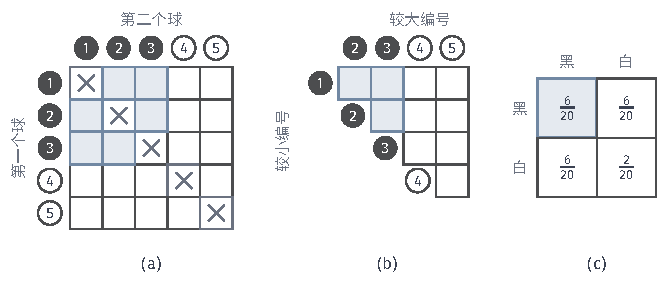
\includegraphics[width=112mm]{figures/07-probability/01-elementary-probability/tikz/cprob-urn-records/figure.pdf}
  \caption{不放回摸两个球的三种记录。实心圆是黑球$1,2,3$，空心圆是白球$4,5$；浅蓝格子是事件“两个都是黑球”。(a)有序对：行是第一个球，列是第二个球，对角线上的格子不可能出现，共$20$个结果。(b)无序对：只保留编号较小者在行、较大者在列的$10$个格子。(c)颜色记录：行、列分别是第一、第二个球的颜色，格中数字是(a)中相应格子数占$20$的比例，四个结果并不同样可能。}
  \label{fig:cprob-urn-records}
\end{BookInlineFigure}

选择样本空间要满足两个要求。第一，它必须细到能表达所关心的事件。事件“第一个球是黑球”在有序记录中是$12$个有序对，在无序记录中却写不出来：子集$\{1,4\}$既可能是先摸到$1$，也可能是先摸到$4$。第二，它最好让每个样本点同样可能，这样概率才能靠计数得到。

颜色记录满足第一个要求，却不满足第二个：图~\ref{fig:cprob-urn-records}(c)中“白白”只对应$2$个有序对，“黑黑”对应$6$个。下一节把“同样可能”写成模型假设，并说明为什么有序记录满足它而颜色记录不满足。

若改为放回摸球，即摸出一个球记下编号后放回盒中，再摸第二个，那么第二个球可以与第一个相同，有序记录的样本空间就是全部$5\times5=25$个有序对，图~\ref{fig:cprob-urn-records}(a)中对角线上的$5$个格子也成为可能结果。放回与否改变的是样本空间本身，而不只是某个事件。
